% Modelling infectious disease dynamics towards informed public-health interventions, with application on \textsc{covid}-19 and cholera.
\chapter*{Introduction} % broad introductio
\addcontentsline{toc}{chapter}{Introduction}
\markboth{Introduction}{}
%epidemics as phenomena
 %d  unevenly distributed among populations. 
 % improverished communties around the world. %public health issue in many countries, and it's elimination of Global North countries -- . 
 %\section{Context}
 Centuries after the first cholera pandemics and 160 years after the realisation that safe drinking-water, adequate sanitation and hygiene prevent its transmission, cholera remains a threat to millions living in hotspots or at risk areas. And the recent emergence of the new coronavirus disease 2019, \textsc{covid}-19, and the strain it put on even world's most advanced healthcare systems recalls the constant risks posed by emerging diseases. Public-health policies have proven the effectiveness of interventions against infectious diseases, showing that deaths are preventable, and sometimes elimination possible. The control of infectious diseases presents challenges accross every dimensions of environmental and human health; in order to prevent spillover events, to block transmission routes, and to protect and treat every person adequately and equally. 

In the fight against infectious diseases, a serie of successes -- attributable to \eg hygiene, vaccines, antibiotics, safe water, ... -- brough the hope of a global and durable reduction of the burden, and a road towards elimination for many diseases. Especially in privileged communities, long-term improvements have been achieved for many of the diseases that have shape the history of humanity. While these progresses show that infectious diseases are not a necessary fate, setbacks on the control of existing and emerging pathogens remind us the ongoing threat they poses on public-health. Indeed, the current global health picture is marked by inequalities in the distribution of the burden, which disproportionaly piles up on already impoverished communities, in conflict zone or after natural disasters. To date, communicable diseases cause approx. 15\% of global deaths every year\cite[-4\baselineskip][tab. 1, excl. non-transmissible neonatal and maternal diseases and nutritional diseases; pre-\textsc{covid}-19 estimates]{Roth:GlobalRegionalNational:2018}, and nearly 1/3 of all child deaths are caused by pneumonia and diarrhoea alone\cite[][\ie 2\textsc{M} deaths among under 5, every year.]{WHO:EndingPreventableChild:2013}.
 
Epidemics -- the rapid spread of an infectious diseases in a population -- are  complex phenomena, the results of interactions between pathogens, environment, societies and individuals\cite{Rinaldo:RiverNetworksEcological:2020a, Buckee:ThinkingClearlySocial:2021, Heesterbeek:ModelingInfectiousDisease:2015}. Public-health policies strive to save lives by designing effective mitigation measures. One of the challenges of designing these policies is dealing with the uncertainties that plague every facet of disease transmission. Only biased and sometime scarce information is available to reason on complex systems with multi-factorial interactions.

%Models are conceptual representations that guide our reasoning about the world.
Models -- conceptual representations of systems -- are tools for us to reason about the world. Historically, conceptual models of the propagation of diseases, from divine retribution to miasma theory, has motivated more (quarantine) or less (persecution) effective approaches to the control of these pests. Scientific breakthroughs in biology and medicine, with the identification of pathogens and their transmission routes, opened the path for improved prevention and treatments. Novel statistical modeling approaches\cite[-3\baselineskip]{Freedman:AssociationCausationRemarks:1999} developed in the 20th century -- and continuously improved ever since\cite{Gelman:WhatAreMost:2021} --  provide a formal framework to reasons about the propagation of a disease in a population. Models enable one to deal with biases on data collection, to account for epistemic uncertainties, to encompass uncertainties in the transmission dynamics. It becomes possible to simulate the disease spread in the affected populations and to study the impact of intervention policies in a principled way. The toolbox was further re-enforced by advances in mechanistic modeling applied to disease transmission, starting from SIR compartmental models\cite{Kermack:ContributionMathematicalTheory:1927, Anderson:PopulationBiologyInfectious:1979}, which divide the population depending on their status with respect to the disease. Later, advances in computing power proved a paradigm shift in dealing with the available evidence, and in representing and inferring features. 

The present thesis explores compartmental models as an approach to infectious disease transmission, and as tools to guide intervention strategies. In each of the presented research work, it is strove to answer a series of research questions, which are variations of: why infectious diseases spread ? and how to prevent them from spreading ? It answers these questions using extensively computer-age modeling and inference methods, in a interactive process represented in fig.~\ref{fig:modeling}. %cyclical pricess cycle: model design, inference, evaluation, results, communication, listening and an important feedback loop.

\begin{figure*}\centering
  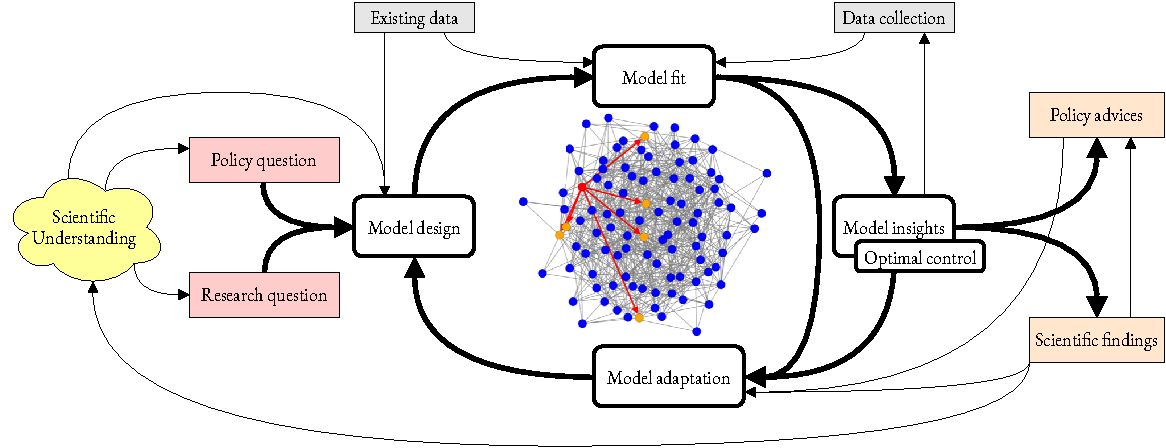
\includegraphics{fig/modeling_cycle_new}
  \caption[Process for infectious disease modeling][-1\baselineskip]{Process for developing models of infectious diseases, with important feedback loop on model results. Apart from data collection, all boxes were explored in the present thesis. The central figure of an agent-based model of disease transmission in a random graph was made by Thomas Fry,  master student supervised during this thesis (with permission).}\label{fig:modeling}
\end{figure*}

TODO DESCRIPTION FIGURE (statistical inference is the global)
An epidemiological model considers different transmission processes which should mimic what we know about the disease and that are relevant for policy makers and/or the research question
.
While designing models, choices on what to include and how to express the supposed dynamics depends on the underlying knowledge of the processes and the available data. 

Once a model has been built, (something else than) statistical inference conditions the model on the observed data. It allows to infer unobserved quantities from reported ones, such as a lockdown intervention from hospitalization and deaths. 
espite its recent formalism, statistical inference remains an art, uncomfortably dependent on the practitioners and their backgrounds\sidenote[][8\baselineskip]{Multimodeling studies and collaborative experiments strive to mitigate this issue by bringing together assumption and projections by different groups. See \eg \url{covid19forecasthub.org/community}}.

After an evaluation of the \textit{fit} of the model and the implication on the results, if the predictive accuracy is satisfying, comes the time to answer the research questions. For example, several models might be compared to identify which transmission routes are responsible for an epidemics, is this case the model is assumed to replicate mechanistic relationships between the component of the real system.

If the model accurately reproduces observed and expected dynamics, it may be used as substitute for experiments, to simulate intervention scenarios and to evaluate the impact of hypothetical policies on a virtual system. In this case it assists one to determine the range of expectations one may have with with regard to real world consequences of tested policies. The communication of model results, with proper awareness of limitation and scope finally provides the opportunity for feedback and eventual adaptation of the model\cite{Heesterbeek:ModelingInfectiousDisease:2015}.

Another application of epidemiological models explored in this thesis is their integration with optimal control methods to search for the \textit{best} intervention against infectious diseases. Optimal control methods are novel mathematical optimization procedure extending the calculus of variations to enable the derivation of control policies. While technical adaptations are necessary to allow its use on epidemics, this rigorous framework identifies the most effective control measures under a set of operational constraints, discovering non-intuitive features and policies. These optimal interventions exploit every features of the complex interactions modelled, allowing to \eg best allocate a limited vaccine supply in space. Such tools, at their infancy and requiring accurate models, are promising as reasoning aid, uncovering another facet of disease transmission, and for effective control of an epidemics.
\begin{table*}[t]
\label{tab:allmodels}
\centering\small
\begin{tabularx}{\textwidth}{x{14mm}cccx{15mm}cx{15mm}p{30mm}}
\toprule
   \small{\textsc{Chapter}}     & Disease           & Comparments & Processes         & \small{$N_{\text{spatial}}$} & Fit       & Aim            & Reference\\
\midrule
4 & Cholera           & SEIR+B      & Stochastic    & --           & MIF-like  & explain         & \tiny{\fullcite{Lemaitre:RainfallDriverEpidemic:2019}}\\
4 & Cholera           & SEIR+B      & Deterministic & --             & MCMC-like & explain        & \tiny{\fullcite{Lemaitre:RainfallDriverEpidemic:2019}}\\
5  & Cholera           & SEAIR$^3$+V & Stochastic    & 10        & MIF-like   & project (scenarios)       & \tiny{\fullcite{Lee:AchievingCoordinatedNational:2020}} \\ \addlinespace
6  & \textsc{\textsc{covid}}-19 & SEI$^3$R+VH & Stochastic    & 3’000+    & MCMC-like & project (scenarios)        & \tiny{\fullcite{Lemaitre:ScenarioModelingPipeline:2021}} \\
7  & \textsc{\textsc{covid}}-19  & SEI$^3$R+H  & Stochastic    & --             & MIF-like  & infer           & \tiny{\fullcite{Lemaitre:AssessingImpactNonpharmaceutical:2020}}\\
8  & \textsc{\textsc{covid}}-19  & SEIAR+VH    & Deterministic & 107       & MCMC-like & optimal\newline control & \tiny{\fullcite{Lemaitre:OptimizingSpatiotemporalAllocation:2021}}\\ 
\bottomrule
\end{tabularx}
\caption[Summary of the models described in this thesis]{Summary of the compartmental models described in this thesis. In column Compartments, the letters indicate the main compartments of the considered model: in addition to susceptible S, exposed (incubating) E , infected (infectious, symptoms) I, infected (infectious, no symptoms) A and recovered R, it is indicated by H the additional compartments to represent the healthcare facilities (hospitalisation, ICUs), by V compartments for vaccinated individuals, and by B the modeling of an environmental reservoir for the bacteria. The exponents denote the number of sub-compartments of that type used to model non-exponential distributions of the residence times in that compartment, using the linear-chain trick. Two fitting procedures are used through the thesis: frequentist iterated filtering and Bayesian Markov-Chain-Monte-Carlo.}
\end{table*}
%\section{Aim and outline}
The present thesis has been developed within the Swiss National Foundation project ``Optimal control of intervention strategies for waterborne disease epidemics (\textsc{snf} 200021–172578)’’. It initial goal was to develop a decision support system for the real-time design of optimal intervention strategies against cholera, which includes an operational forecasting tool coupled with an optimal control solver. This framework has been developed, albeit for \textsc{covid}-19 transmission in Italy, and is presented in \textsc{Chapter 6}. Indeed the \textsc{covid}-19 pandemic has disrupted the research plan of the present thesis. As a consequence, it happens to associate two antipodean diseases. Cholera, one of the most ancient recorded disease\footnote[][10\baselineskip]{History of pre-pandemic cholera is uncertain but numerous accounts of the disease are supposed from as early as 400\textsc{bce}. See \fullcite[p. 95]{Byrne:EncyclopediaPestilencePandemics:2008}.}, has caused 7 pandemics in the modern era. In contrast, \textsc{covid}-19 earliest known onset of symptoms is on December 1, 2019. The pathogen for cholera is a bacteria, \textit{Vibrio Cholerae}, responsible for heavy watery diarrhea, whereas \textsc{SARS-CoV-2}, \textsc{covid}-19’s pathogen, is a virus responsible for respiratory infections. Cholera belongs to the negletected tropical diseases, a class of understudied infections while the \textsc{covid}-19 pandemic has sparked an unprecedented accumulation of evidence\sidenote[][]{With more than 190'000 peer-reviewed papers and many more preprints, website and reports published at the time of writing. Estimation from: \fullcite{COVID-19OpenAccessProject:LivingEvidenceCOVID19:2020}}. 
Other differences between the two disease include the posited transmission routes (fecal-oral vs. respiratory route), the affected communities (``poorest of the poor”, higher severity on children vs. global, higher severity on elders), etc... Despite these differences, cholera and \textsc{covid}-19 shares mechanisms that makes their transmission sustainable in populations and causes pandemics with a regretfully high toll on human lives, and a distribution of burden that echoes unequal access to care and disproportionately affects stigmatized communities. Both cholera and \textsc{covid}-19 are infectious diseases -- with the potential of starting epidemics and pandemics, and the many of the scientific methods to study the spread and interventions are shared across these diseases and others.


A set of 5 models, see tab.~\ref{tab:allmodels}, is proposed in this thesis, with features that depends on the disease, the context, the possible control measures and the uncertainties associated with the data and the processes. Some models have stochastic transitions, others are mostly deterministic, some models consider human mobility across regions whereas others assume well-mixed population. Despite the foregoing differences, all the models presented in this thesis are compartmental with some mechanistic components; all are based on the SIR model.

The work presented extensively builds on the ECHO laboratory expertise on the spatially-explicit modeling of cholera transmission\footnote{and waterborne diseases in general; see: \fullcite{Rinaldo:RiverNetworksEcological:2020a, Rinaldo:Reassessment20102011:2012}}. The group has developed over a decade a rainfall-mediated, spatially explicit cholera model that has inspired each of the other models presented in this thesis. The original model developed in the group, is presented in \textsc{Chapter 1}, with a short introduction on the ancient disease that is cholera, and its sorrowful history.

Cholera is the focus of two additional chapters. The explanatory power of two existing models of cholera transmission and its link to rainfall are compared in \textsc{Chapter 2}, through the analysis of an outbreak in Juba, South-Sudan. In \textsc{Chapter 3}, a scenario planning estimation of the probability of eliminating cholera from Haiti with a mass vaccination campaign is presented; this work has been carried within the framework of a multi-modeling study with other groups, and input from the ministry of health of Haiti.
\marginnote[-5\baselineskip]{Most bibliographic items and some additional precision are presented as margin notes for convenience. However, the full bibliography is included at the end of the thesis.}
The remaining chapters focus on \textsc{covid}-19. In \textsc{Chapter 4} some facets of dealing with uncertainties from the early days of the pandemic are uncovered, with a focus on a pipeline for scenario modeling that has been used to inform governments, in the United States and other countries. 
An inference study to estimate the impact of the interventions against \textsc{covid}-19 in Switzerland is presented in \textsc{Chapter 5}.
%\marginnote[-5\baselineskip]{Incidentaly, this organisation reflects the chronogical order of the work.}
Finally, \textsc{Chapter 6} presents how to integrate a spatially explicit epidemiological model for the Italian epidemic within an optimal control framework in order to discover the optimal strategy for vaccine allocation.

